\chapter*{Abstract}
\addcontentsline{toc}{chapter}{Abstract}

Current \acp{BAS} have crucial context-awareness limitations that must be addressed before they can reach human-like levels and better adapt to the dynamic needs of modern buildings. Among others, our buildings still lack sensors, actuators, and control agents that learn reliable models of the environment and plan complex action sequences. Moreover, modern \ac{ML}-backed \acp{BAS}, though trained on massive datasets, are usually overly specialized (trained for one task) and brittle (make stupid mistakes). In contrast, human learning is very efficient and with only a few examples, we can find intuitive ways to complete a task while generalizing our learning to other tasks. To address the above limitations, this thesis proposes a foundational framework that advances the context-awareness capabilities of \acp{BAS} using knowledge graphs and \ac{KRL}. At the framework's core is the notion of using \ac{SWT} to model the semantic relationships between different building components, packaging them inside a network-like data structure called a \ac{BIM}-based Knowledge Graph (BIM-KG)\footnote{Knowledge graphs derived from \ac{BIM} with the help of \acp{SWT} are referred to as \acp{BIM-KG} for the remainder of this thesis}, and using \ac{KRL} to learn the hidden patterns within the \ac{BIM-KG}. During the learning phase, \ac{KRL} utilizes message-passing to propagate the learnt information throughout all nodes in the \ac{BIM-KG}. This research hypothesizes that building automation agents can leverage this notion of message-passing to aggregate contextual information from all entities in a \ac{BIM-KG} and use it to continuously update their understanding of a building's systems and components. The perception is that imbuing building automation agents with holistic information about the buildings they control can support context-aware decision-making during downstream automation tasks.

To test the research hypothesis, a three-phase investigation was carried out: literature review, framework development, and framework applicability. Phase one focused on \textit{situating the research} within the scholarly discourse of \ac{BIM}, \acp{BIM-KG}, building automation, and \ac{KRL}. The results show that since the advent of \ac{SWT} in the \ac{AEC/FM} field in 2010, it has been a driving force in advancing \ac{BIM} research by providing the mechanics to represent complex relationships within the built environment. Concurrently, \ac{KRL} has seen significant development in domains such as bioinformatics, where it has been used to understand complex biological relationships and processes; however, despite the apparent suitability of applying \ac{KRL} to the \ac{BIM} field, such integration has not materialized and remains largely unexplored. To get around these research shortcomings, the next phase of this thesis was to \textit{develop a framework} for applying \ac{KRL} to \acp{BIM-KG} using performance analysis experiments. Five baseline \ac{KRL} models were chosen for this. The chosen models are well-regarded techniques from existing studies, cover a wide range of methodologies, and have been extensively investigated in the context of drug discovery, whose data structures closely mirror those of \acp{BIM-KG}. Two publicly available \acp{BIM-KG} datasets were used in these experiments. The overall goal was not to identify the best \ac{KRL} model configurations. Instead, the study examined more closely how model performance can be affected by modifications to the training step, selection of hyper-parameters and their optimization. The experimental results were used to define the prerequisites for integrating \ac{KRL} with \acp{BIM-KG} in a domain-independent framework.
This means that although a building automation use case is used to formulate the framework, it can be applied to other \ac{AEC/FM} domains such as heritage, quantity-takeoff and energy analysis. The experimental findings show that RotatE and TransE consistently outperform other models across both datasets, establishing themselves as robust baselines when integrating \ac{KRL} with \acp{BIM-KG}. It is also interesting to see that older models like TransE can still be competitive with optimized training and \ac{HPO} configurations. Adam and NSSA emerged as favourable training setup choices, suggesting their potential as initial benchmarks for future evaluations. Despite extensive hyper-parameter searches, there was considerable variance among top-performing model configurations, indicating the need for nuanced parameter combinations. This complexity suggests that manual tuning may not yield optimal results, advocating for the adoption of \ac{HPO} strategies. Furthermore, the disparity in hyper-parameters between the two datasets underscores the influence of dataset-specific parameters. Finally, random search methods, when repeated sufficiently, yield configurations closely comparable to more systematic approaches, albeit in less time.

\textit{To illustrate the feasibility of the framework}, phase three devises a setup consisting of a \ac{BIM} model, \ac{IoT} devices, and a prototype program of the framework wrapped inside an \ac{API}. The \ac{API} consists of a server-side module and a client-side module. The server-side module demonstrates how a building automation system can communicate with \ac{KRL} configurators, external services such as \ac{BIM-KG} databases, sensor data stores, and \ac{MQTT} brokers. The client-side module consists of a \ac{GUI} with \ac{COBie} handler service that facilitates the curation of \acp{BIM-KG} from \ac{COBie} files and an interrogation service that facilitates declarative interrogation of the server-side module using \ac{SPARQL} and \ac{GraphQL}. For \ac{KRL} to impact the \ac{AEC/FM} domain, this work emphasizes the critical importance of comprehensively reporting model architectures, training setups, hyperparameters, and dataset splits to enhance trust, reproducibility and understanding of \ac{KRL}-based methods among \ac{AEC/FM} stakeholders and researchers. This insight highlights a prevalent issue in the \ac{AEC/FM} field where results are often difficult to replicate due to incomplete documentation of experimental setups.

% \section*{Graphical Abstract}
% \begin{figure}[!h]
%     \centering
%     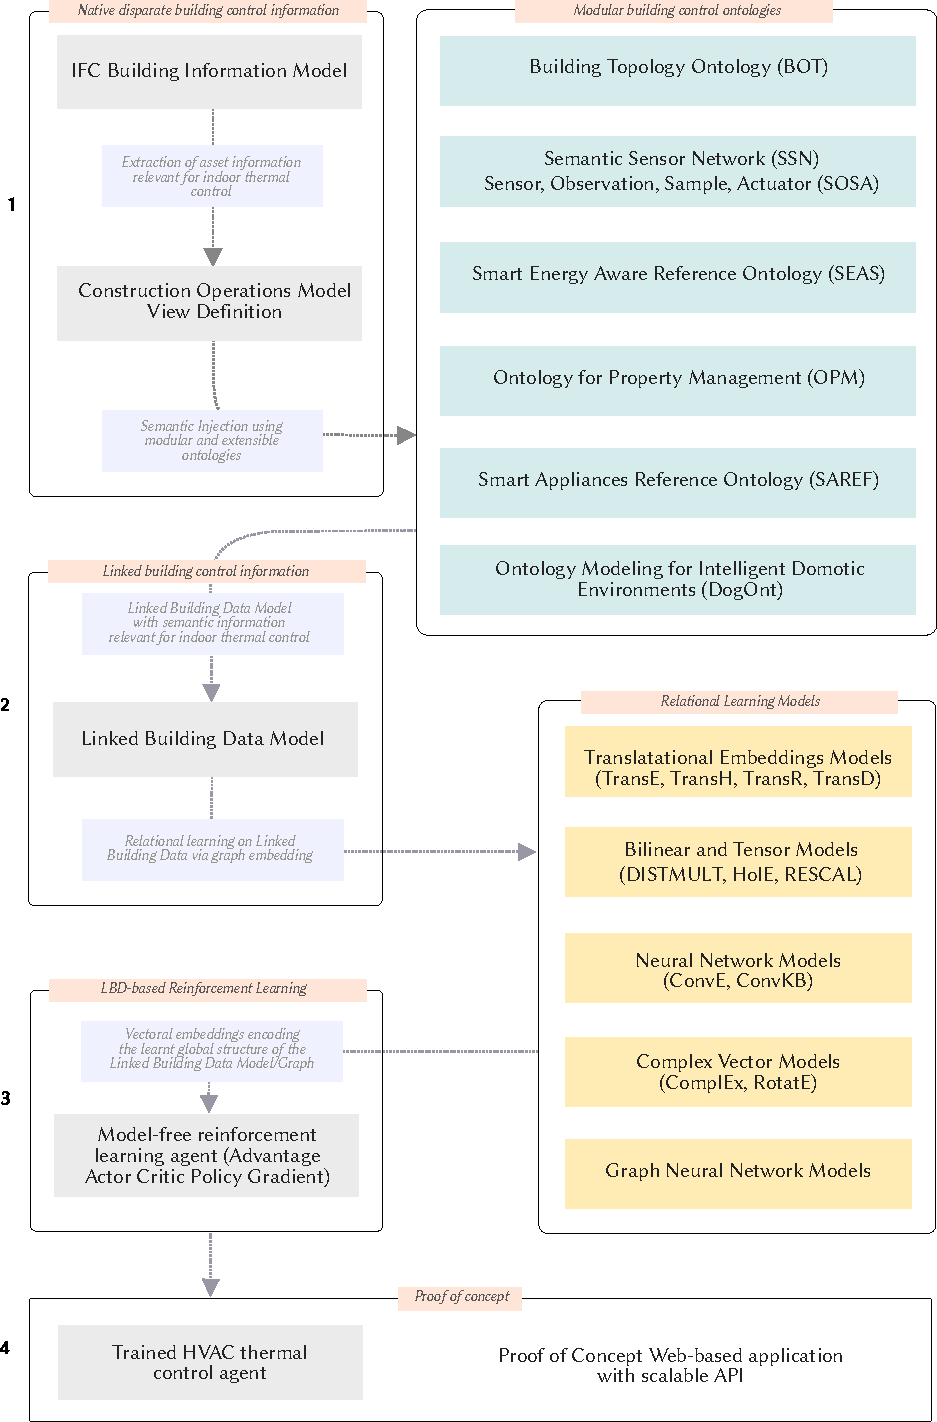
\includegraphics[width=\textwidth]{figures/graphabstract.pdf}
%     \caption{Graphical abstract of the research work herein} \label{Graphical abstract}
% \end{figure}

